\section{Otimiza\c{c}\~{a}o e Engenharia de Reservat\'{o}rio}
\subsection{Contexto}
Na engenharia de reservat\'{o}rios, os pesquisadores buscam m\'{e}todos visando \`{a} melhoria das condi\c{c}\~{o}es e resultados produtivos dos reservat\'{o}rios existentes. Atualmente, estima-se que at\'{e} 60\% de \'{o}leo podem ser recuperados a partir do emprego de t\'{e}cnicas de EOR \footnote{Informa\c{c}\~{a}o dispon\'{i}vel em <http://energy.gov/fe/science-innovation/oil-gas-research/enhanced-oil-recovery>. Acesso em: 17 de Setembro de 2018}. De acordo com Udy \textit{et al.}, m\'{e}todos de EOR e de inje\c{c}\~{a}o de \'{a}gua s\~{a}o utilizados, a depender das propriedades e do estado de produ\c{c}\~{a}o do reservat\'{o}rio, de maneira a se encontrar condi\c{c}\~{o}es \'{o}timas de produ\c{c}\~{a}o de \'{o}leo ou de NPV \cite{udyEOR}.

Geralmente, os engenheiros de reservat\'{o}rio e de produ\c{c}\~{a}o buscam encontrar aloca\c{c}\~{o}es de recursos de produ\c{c}\~{a}o por meio de simula\c{c}\~{o}es computacionais baseadas na estrat\'{e}gia de tentativa e erro; contudo, tal abordagem reduz a probabilidade de se encontrar as condi\c{c}\~{o}es \'{o}timas de produ\c{c}\~{a}o, uma vez que poucos cen\'{a}rios s\~{a}o considerados. Al\'{e}m disso, como \'{e} invi\'{a}vel a obten\c{c}\~{a}o de uma grande quantidade de simula\c{c}\~{o}es, os resultados conduzem a condi\c{c}\~{o}es n\~{a}o otimizadas e redu\c{c}\~{a}o da produ\c{c}\~{a}o total. Al\'{e}m das limita\c{c}\~{o}es computacionais, outros desafios se tornam presentes na otimiza\c{c}\~{a}o da produ\c{c}\~{a}o de petr\'{o}leo, a saber: a falta de dados hist\'{o}ricos adequados para a calibra\c{c}\~{a}o do modelo matem\'{a}tico, as discrep\^{a}ncias presentes nos par\^{a}metros f\'{i}sicos, a imprevisibilidade dos pre\c{c}os do \'{o}leo e do g\'{a}s, entre outros\footnote{Ver \cite{udyEOR}}.

No esfor\c{c}o de se encontrar as melhores condi\c{c}\~{o}es de opera\c{c}\~{a}o de reservat\'{o}rios, foram feitas tentativas de se desenvolver simuladores que conseguissem obter os melhores esquemas de produ\c{c}\~{a}o, combinando simula\c{c}\~{o}es de reservat\'{o}rio com algoritmos de busca linear; entretanto, simuladores baseados em diferen\c{c}as finitas possuem uma multitude de vari\'{a}veis e rela\c{c}\~{o}es que n\~{a}o se integram facilmente aos m\'{e}todos num\'{e}ricos de otimiza\c{c}\~{a}o. A chave para o m\'{e}todo proposto \'{e} se obter uma diferencia\c{c}\~{a}o total do simulador, assim tornando-se poss\'{i}vel a computa\c{c}\~{a}o eficiente e precisa de buscas de gradiente direcional \cite{asheim88}. 

No campo da engenharia de reservat\'{o}rio, s\~{a}o utilizados tanto algoritmos de gradiente descendente quanto meta-heur\'{i}sticos na resolu\c{c}\~{a}o de problemas de otimiza\c{c}\~{a}o. Ser\~{a}o analisadas duas classes de problemas envolvendo reservat\'{o}rios: maximiza\c{c}\~{a}o da produ\c{c}\~{a}o de \'{o}leo e do NPV, e posicionamento de po\c{c}os.
\nocite{EOR:Intro}


\subsection{Algoritmos de Gradiente Descendente}
O uso de algoritmos de gradiente descendente est\'{a} bastante difundido na engenharia de reservat\'{o}rios, em particular em situa\c{c}\~{o}es em que se busca otimizar a produ\c{c}\~{a}o e o NPV. Fonseca \textit{et al.}, por exemplo, utiliza varia\c{c}\~{o}es estoc\'{a}sticas do algoritmo simplex, de maneira a se lidar com as incertezas de simula\c{c}\~{a}o e, assim, buscar o resultado \'{o}timo, comparando a solu\c{c}\~{a}o proposta com algoritmos de otimiza\c{c}\~{a}o robusta \cite{fonseca}; Asheim descreve um algoritmo utilizando busca linear em conjunto com as condi\c{c}\~{o}es KKT, calculando sucessivamente o NPV durante o algoritmo, ilustrado pela Figura \ref{fig:asheim1} \cite{asheim88}.

\begin{figure}[H]
	\centering
	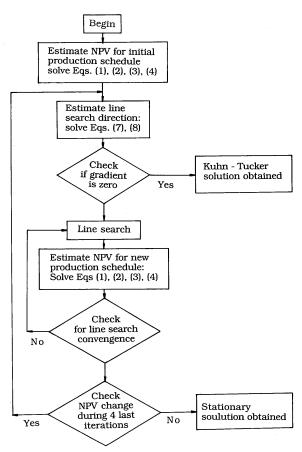
\includegraphics[width=.5\textwidth]{figs/revisao/revisao_asheim1}
	\caption{Exemplo de algoritmo de gradiente descendente aplicado para NPV \cite{asheim88}\label{fig:asheim1}}
\end{figure}

Os algoritmos envolvendo gradientes podem tamb\'{e}m ser acrescidos de m\'{e}todos adjuntos; Essen \textit{et al.}, por exemplo, usam esses m\'{e}todos em conjunto com um algoritmo de otimiza\c{c}\~{a}o robusta aplicado a um conjunto de 100 realiza\c{c}\~{o}es de um reservat\'{o}rio\footnote{Ver \cite{SPE:RWO}.}, enquanto que Liu e Reynolds utilizam um NBI (\textit{Normal Boundary Intersection}) com uso de uma fun\c{c}\~{a}o Lagrangiana aumentada, em que os gradientes necess\'{a}rios s\~{a}o computados por m\'{e}todos adjuntos \cite{GEO:LIU}; nesse \'{u}ltimo caso, dois problemas envolvendo inje\c{c}\~{a}o de \'{a}gua foram considerados: o primeiro problema almejava maximizar o NPV da vida \'{u}til do reservat\'{o}rio e o NPV a curto prazo; j\'{a} o segundo problema, aplicado a uma descri\c{c}\~{a}o incerta de um reservat\'{o}rio, tinha como objetivo maximizar o valor esperado do NPV durante o ciclo de produ\c{c}\~{a}o do reservat\'{o}rio e diminuir o desvio padr\~{a}o do NPV em um conjunto de realiza\c{c}\~{o}es geol\'{o}gicas\footnote{Ver \cite{GEO:LIU}.}.

Outros algoritmos considerados de gradiente descendente, al\'{e}m dos j\'{a} descritos, s\~{a}o utilizados tamb\'{e}m em problemas envolvendo inje\c{c}\~{a}o de \'{a}gua; Asadollahi e N{\ae}vdal, por exemplo, utilizam uma combina\c{c}\~{a}o do m\'{e}todo da descida r\'{a}pida com o gradiente conjugado com vistas \`{a} maximiza\c{c}\~{a}o da produ\c{c}\~{a}o. A solu\c{c}\~{a}o obtida \'{e} ent\~{a}o testada em outras realiza\c{c}\~{o}es do mesmo reservat\'{o}rio, obtidas por meio de ajuste de hist\'{o}rico, de maneira a se testar a robustez da mesma \footnote{Ver \cite{SPE:WFO}.}. Al\'{e}m dos m\'{e}todos j\'{a} citados, outro algoritmo presente na literatura \'{e} o SQP: Grema \textit{et al.} utilizam o SQP em um reservat\'{o}rio cujo modelo, resultante de uma identifica\c{c}\~{a}o, \'{e} uma rede neural do tipo NARX (\textit{Nonlinear Autoregressive with Exogenous Input})\footnote{O modelo NARX pode ser encontrado em \cite[p. 390]{aguirre}.}; a simula\c{c}\~{a}o foi conduzida com uso do MRST \cite{grema2017optimization}. J\'{a} Lorentzen \textit{et al.} usam o SQP em conjunto com um Filtro de Kalman especial, denominado \textit{Ensemble Kalman Filter} --- o filtro \'{e} utilizado durante a assimila\c{c}\~{a}o dos dados, e o SQP \'{e} destinado \`{a} obten\c{c}\~{a}o do NPV \'{o}timo, sendo o n\'{u}mero de vari\'{a}veis do problema inicialmente reduzido \cite{lorentzen2009sqp}.

Os problemas envolvendo posicionamento de po\c{c}os, ao contr\'{a}rio da otimiza\c{c}\~{a}o por meio do NPV, possuem menor n\'{u}mero de publica\c{c}\~{o}es em que s\~{a}o utilizados m\'{e}todos envolvendo gradientes; Sarma e Chen explicam esse fato partindo da premissa que as posi\c{c}\~{o}es dos po\c{c}os s\~{a}o discretas, e que o gradiente da fun\c{c}\~{a}o objetivo em respeito a esses par\^{a}metros n\~{a}o \'{e} definido; contudo, os mesmos autores descrevem uma adapta\c{c}\~{a}o do problema em que a fun\c{c}\~{a}o de posicionamento dos po\c{c}os \'{e} adaptada para um modelo cont\'{i}nuo, possibilitando o uso de algoritmos de gradiente descendente. Ainda assim, eles destacam que, em problemas de posicionamento de po\c{c}os, os algoritmos mais utilizados s\~{a}o os meta-heur\'{i}sticos \cite{sarmaChen}.


\subsection{Algoritmos Meta-heur\'{i}sticos}
Al\'{e}m dos algoritmos de gradiente descendente, os m\'{e}todos meta-heur\'{i}sticos de otimiza\c{c}\~{a}o est\~{a}o bem difundidos na literatura, no que diz respeito \`{a} resolu\c{c}\~{a}o tanto de problemas de obten\c{c}\~{a}o de condi\c{c}\~{o}es \'{o}timas de produ\c{c}\~{a}o quanto de posicionamento inteligente de po\c{c}os. Entre os algoritmos utilizados, destacam-se os algoritmos gen\'{e}ticos (GA), o PSO, o \textit{simulated annealing} (SA), entre outros.

Em problemas de otimiza\c{c}\~{a}o da produ\c{c}\~{a}o, notadamente em esquemas de explota\c{c}\~{a}o envolvendo o uso da inje\c{c}\~{a}o de \'{a}gua, os algoritmos gen\'{e}ticos t\^{e}m destaque: Mamghaderi e Pourafshary buscam maximizar a produ\c{c}\~{a}o de \'{o}leo alocando volumes de \'{a}gua nos injetores, utilizando um algoritmo gen\'{e}tico em conjun\c{c}\~{a}o com um modelo capacitor-resistor (CRM)\footnote{O CRM \'{e} explicado e utilizado em \cite{SAYARPOUR2009227}.} \cite{MAMGHADERI2013107}; Safarzadeh \textit{et al.} utilizam tanto um GA quanto uma vers\~{a}o multi-objetivo do mesmo (MOGA) com vistas \`{a} obten\c{c}\~{a}o de um esquema \'{o}timo de inje\c{c}\~{a}o de \'{a}gua, reduzindo alguns efeitos como a perda do fluido injetado para os aqu\'{i}feros e a produ\c{c}\~{a}o indesejada de \'{a}gua \cite{Safarzadeh2015}.

Al\'{e}m dos algoritmos gen\'{e}ticos, o \textit{simulated annealing} tamb\'{e}m encontra espa\c{c}o nos problemas de otimiza\c{c}\~{a}o dos esquemas de produ\c{c}\~{a}o. Yang \textit{et al.} argumentam que o SA e o GA podem ser utilizados para se extender a vida \'{u}til do reservat\'{o}rio e aumentar a rentabilidade \cite{YANG200369}. J\'{a} Khan \textit{et al.} mostram que \'{e} poss\'{i}vel, utilizando o SA com restri\c{c}\~{o}es, maximizar a vaz\~{a}o de \'{o}leo a curto prazo e a recupera\c{c}\~{a}o a longo prazo em esquemas de inje\c{c}\~{a}o de \'{a}gua \cite{khanSA}. Outro algoritmo meta-heur\'{i}stico utilizado na otimiza\c{c}\~{a}o da produ\c{c}\~{a}o \'{e} o PSO: Siavashi e Yazdani fazem um estudo comparativo entre o PSO, o GA e algoritmos h\'{i}bridos no que concerne \`{a} otimiza\c{c}\~{a}o aplicada em esquemas de inje\c{c}\~{a}o de \'{a}gua \cite{siavashiPSO}. Ademais, Sorek \textit{et al.} utilizam o PSO na busca por um controle \'{o}timo mais suave dos po\c{c}os, sem prejudicar o custo computacional \cite{Sorek2017}.

Os algoritmos meta-heur\'{i}sticos s\~{a}o largamente empregados, tamb\'{e}m, em problemas de posicionamento dos po\c{c}os; como destacam Sarma e Chen, eles s\~{a}o a solu\c{c}\~{a}o mais utilizada nesse tipo de problema devido \`{a} natureza da fun\c{c}\~{a}o objetivo: o posicionamento dos po\c{c}os \'{e} enxergado como uma fun\c{c}\~{a}o discreta de coordenadas cartesianas \cite{sarmaChen}. Montes \textit{et al.} ainda identificam a inviabilidade do uso de algoritmos baseados em gradiente para resolver problemas de posicionamento devido \`{a}s descontinuidades e n\~{a}o-linearidades da fun\c{c}\~{a}o objetivo; os mesmos apresentam o uso de algoritmo gen\'{e}tico para a obten\c{c}\~{a}o de uma boa solu\c{c}\~{a}o para o problema proposto \cite{montesETAL}. O uso de algoritmos gen\'{e}ticos \'{e} tamb\'{e}m proposto por Farshi\footnote{Farshi tamb\'{e}m considera a exist\^{e}ncia do requisito de dist\^{a}ncia Euclidiana m\'{i}nima dos po\c{c}os \cite{farshi}.} e Bukhamsin \textit{et al.}\footnote{Os referidos autores realizaram o algoritmo sobre um campo real no Oriente M\'{e}dio, considerando geometrias de po\c{c}os complexas, como po\c{c}os multilaterais \cite{bukhamsin}.} na sua varia\c{c}\~{a}o cont\'{i}nua. Outros usos do GA incluem os trabalhos propostos por Emerick \textit{et al.}\footnote{Trata-se do uso de um GA para otimiza\c{c}\~{a}o de posicionamento de po\c{c}os com restri\c{c}\~{o}es n\~{a}o-lineares \cite{emerick}.} e Min \textit{et al.}; neste \'{u}ltimo, \'{e} utilizada a vers\~{a}o multi-objetivo, o MOGA, para se obter o posicionamento de po\c{c}os injetores, sobre um modelo simulado com \textit{black oil}. 

Outro algoritmo utilizado para o problema de posicionamento dos po\c{c}os \'{e} o SA; Beckner e Song, por exemplo, fazem uma analogia entre o problema de posicionamento e um problema do caixeiro viajante, empregando o SA para obter a solu\c{c}\~{a}o desejada \cite{beckner}. Uma vers\~{a}o alternativa do SA, denominada \textit{Very Fast Simulated Annealing} (VFSA) foi utilizada por Parashar \textit{et al.}\footnote{Ver \cite{parashar}.} e por Banghert \textit{et al.}\footnote{Os autores ainda realizam uma compara\c{c}\~{a}o envolvendo o VFSA e outros algoritmos; ver \cite{Bangerth2006}.}.

Um terceiro algoritmo de otimiza\c{c}\~{a}o bastante utilizado para se obter o posicionamento \'{o}timo dos po\c{c}os \'{e} o PSO: Onwunalu e Durlofsky utilizam o PSO para determinar, al\'{e}m do posicionamento, o tipo dos po\c{c}os \cite{Onwunalu2010}; Nwankwor\textit{et al.} implementam o PSO para se obter o posicionamento \'{o}timo dos po\c{c}os, comparando a solu\c{c}\~{a}o com a resultante de um algoritmo de evolu\c{c}\~{a}o diferencial. Por fim, os autores mesclam os dois algoritmos citados em um m\'{e}todo h\'{i}brido, denominado \textit{Hybrid Particle Swarm Differential Evolution} (HPSDE)\footnote{Ver \cite{Nwankwor2013}.}. O PSO foi tamb\'{e}m utilizado por Ding \textit{et al.}, sendo propostas varia\c{c}\~{o}es do algoritmo, evidenciando o fato de que modifica\c{c}\~{o}es no PSO, aliadas ao uso de um \textit{quality map}, podem levar a melhores resultados de posicionamento \'{o}timo \cite{Ding2014}.

H\'{a} outros algoritmos meta-heur\'{i}sticos que podem ser citados envolvendo posicionamento dos po\c{c}os; o \textit{harmony search}, por exemplo, \'{e} utilizado por Afshari \textit{et al.}, em uma vers\~{a}o melhorada, combinada com simula\c{c}\~{o}es \textit{streamline} \cite{AFSHARI2011664}. Um outro algoritmo, denominado algoritmo dos morcegos (\textit{Bat Algorithm}), foi utilizado por Naderi e Khamehchi para a resolu\c{c}\~{a}o tanto de problemas de posicionamento quanto de controle dos po\c{c}os\footnote{Ver \cite{NADERI2017348} e \cite{NADERI201747}.}; por fim, ser\'{a} citado um algoritmo recente, datado de 2007, denominado \textit{Imperialist Competitive Algorithm} (ICA)\footnote{Ver \cite{ICAdef}}; Al Dossary e Nasrabadi utilizam esse algoritmo para se determinar o posicionamento \'{o}timo dos po\c{c}os, comparando os resultados com os obtidos por PSO e GA \cite{ALDOSSARY2016237}.